\documentclass[25pt, a0paper, portrait, innermargin=4cm, colspace=2.5cm]{tikzposter}
\geometry{paperwidth=80cm}
% load packages
\usepackage[utf8]{inputenc}
\usepackage{mathpazo}
\usepackage[sfdefault,light]{roboto}
\usepackage[T1]{fontenc}
\usepackage{amsmath} 
\usepackage{blindtext}
\usepackage{comment}
\usepackage{enumerate}
\usepackage{xcolor}
\usepackage{boolexpr}
\usepackage{multicol}
\usetikzlibrary{arrows, decorations.markings}

% define default font
\renewcommand{\familydefault}{\sfdefault}

% color definitions
\definecolor{tublue}{HTML}{3571A1}
\definecolor{tulightblue}{HTML}{589DD4}
\definecolor{tuorange}{HTML}{F6C07C}

% block style definitions
\defineblockstyle{myDefault}{titlewidthscale=1, bodywidthscale=1, titleleft, titleoffsetx=0cm, titleoffsety=0cm, bodyoffsetx=0cm, bodyoffsety=-1cm, bodyverticalshift=0pt, roundedcorners=0, linewidth=0.1cm, titleinnersep=0.5cm, bodyinnersep=0cm}
{\begin{scope}[line width=\blocklinewidth, rounded corners=\blockroundedcorners]
    \ifBlockHasTitle
        %\draw[draw=none]
        %    (blockbody.south west) rectangle (blocktitle.north east);
        \draw[color=tulightblue, loosely dotted, line width=1mm]
        (blocktitle.south west) -- (blocktitle.south east);
        %\draw[color=tublue, solid, line width=2mm]
        %([yshift=-2mm]blocktitle.south west) -- ([yshift=-2mm]blocktitle.south east);
    \else
        \draw[draw=none]
            (blockbody.south west) rectangle (blockbody.north east);
    \fi
\end{scope}}

% define title style
\definetitlestyle{myWave}{width=\paperwidth, roundedcorners=0, linewidth=0pt, innersep=1.5cm, titletotopverticalspace=0mm, titletoblockverticalspace=35mm, titlegraphictotitledistance=10pt, titletextscale=2}
{
    \coordinate (topleft) at (\titleposleft,\titlepostop);
    \coordinate (topright) at (\titleposright,\titlepostop);
    \coordinate (lefttoright) at (\titlewidth,0);
    \coordinate (head) at (0,\titlepostop-\titleposbottom);
    \coordinate (bottomright) at (\titleposright,0);
    \coordinate (footerheight) at (0, 9);
    %
    \draw[draw=none, left color=tublue, right color=tublue]%
        (topright) -- %
        (topleft) -- %
        ($(topleft) - (head)$) -- %
        ($(topright) - (head)$) -- cycle; %
    \draw[draw=none, left color=tuorange, right color=tuorange]%
        ($(topright) - (head)$ ) --  %
        ($(topleft) - (head)$) -- %
        ($(topleft) - (head)-(0,.5)$) -- %
        ($(topright) - (head)-(0,.5)$) -- cycle; %
    \draw[draw=none, left color=tulightblue, right color=tulightblue]%
        ($(topright) - (head)-(0,.5)$ ) --  %
        ($(topleft) - (head)-(0,.5)$) -- %
        ($(topleft) - (head)-(0,1.)$) -- %
        ($(topright) - (head)-(0,1.)$) -- cycle; %
    \draw[draw=none, left color=tublue, right color=tublue]%
        ($(topright) - (head)-(0,1.)$ ) --  %
        ($(topleft) - (head)-(0,1.)$) -- %
        ($(topleft) - (head)-(0,1.5)$) -- %
        ($(topright) - (head)-(0,1.5)$) -- cycle; %
    \draw[draw=none, left color=tublue, right color=tublue]%
        (bottomleft) --  %
        ($(bottomleft) + (\titlewidth, 0)$) -- %
        ($(bottomleft) + (\titlewidth, 0) + (footerheight)$) -- %
        ($(bottomleft) + (footerheight)$) -- cycle; %
    \draw[draw=none, left color=tuorange, right color=tuorange]%
        ($(bottomleft) + (footerheight)$) -- %
        ($(bottomleft) + (\titlewidth, 0) + (footerheight)$) -- %
        ($(bottomleft) + (\titlewidth, 0.5) + (footerheight)$) -- %
        ($(bottomleft) + (0, 0.5) + (footerheight)$) -- cycle; %
    \draw[draw=none, left color=tulightblue, right color=tulightblue]%
        ($(bottomleft) + (0, 0.5) + (footerheight)$) -- %
        ($(bottomleft) + (\titlewidth, 0.5) + (footerheight)$) -- %
        ($(bottomleft) + (\titlewidth, 1.) + (footerheight)$) -- %
        ($(bottomleft) + (0, 1.) + (footerheight)$) -- cycle; %
    \draw[draw=none, left color=tublue, right color=tublue]%
        ($(bottomleft) + (0, 1.) + (footerheight)$) -- %
        ($(bottomleft) + (\titlewidth, 1.) + (footerheight)$) -- %
        ($(bottomleft) + (\titlewidth, 1.5) + (footerheight)$) -- %
        ($(bottomleft) + (0, 1.5) + (footerheight)$) -- cycle; %
}

% define color palette
\definecolorpalette{sampleColorPalette} {
  \definecolor{colorOne}{named}{tublue}
  \definecolor{colorTwo}{named}{tuorange}
  \definecolor{colorThree}{named}{tulightblue}
}

% set color styles
\definecolorstyle{sampleColorStyle} {
  \definecolor{colorOne}{named}{blue}
  \definecolor{colorTwo}{named}{yellow}
  \definecolor{colorThree}{named}{orange}
  }{
  % Background Colors
  \colorlet{backgroundcolor}{white}
  \colorlet{framecolor}{white}
  % Title Colors
  \colorlet{titlefgcolor}{white}
  \colorlet{titlebgcolor}{tublue}
  % Block Colors
  \colorlet{blocktitlebgcolor}{white}
  \colorlet{blocktitlefgcolor}{tublue}
  \colorlet{blockbodybgcolor}{white}
  \colorlet{blockbodyfgcolor}{black}
  % Innerblock Colors
  \colorlet{innerblocktitlebgcolor}{white}
  \colorlet{innerblocktitlefgcolor}{black}
  \colorlet{innerblockbodybgcolor}{black}
  \colorlet{innerblockbodyfgcolor}{black}
  % Note colors
  \colorlet{notefgcolor}{black}
  \colorlet{notebgcolor}{colorTwo!50!white}
  \colorlet{noteframecolor}{colorTwo}
}

% define note style
\definenotestyle{myNotestyle}{targetoffsetx=0pt, targetoffsety=0pt, angle=45, radius=8cm, width=6cm, connection=true, rotate=0, roundedcorners=0, linewidth=1pt, innersep=0pt}
{
  \ifNoteHasConnection
      \draw[thick] (notecenter) -- (notetarget)
      node{$\bullet$};
  \fi
  \draw[draw=notebgcolor,fill=notebgcolor,rotate=\noterotate](notecenter.south west) rectangle (notecenter.north east);
}

% define final poster layout
\definelayouttheme{sample}{
  \usecolorstyle[colorPalette=sampleColorPalette]{sampleColorStyle}
  \usebackgroundstyle{sample}
  \usetitlestyle{myWave}
  \useblockstyle{myDefault}
  \useinnerblockstyle{Minimal}
  \usenotestyle{myNotestyle}
}

\usetheme{sample}



\title{An enhanced Soil Moisture product from \\ the ERS Scatterometers}
\author{\underline{Christoph Reimer}, Isabella Pfeil and Wolfgang Wagner}
\date{ESA Living Planet Symposium, 9-13 May 2016, Prague, Czech Republic}
\titlegraphic{
\includegraphics[scale=1]{graphics/TULogo.png}}
\institute{Vienna University of Technology, Department of Geodesy and Geoinformation}

\settitle{
  \begin{center}
    \begin{minipage}[t]{0.95\paperwidth}
        \begin{minipage}{0.18\linewidth}
          \@titlegraphic
        \end{minipage}
        \hfil
        \begin{minipage}{0.6\linewidth}
          \centering
          \color{titlefgcolor}
          {\bfseries \sffamily \Large \@title \par}
          \vspace*{1em}
          {\LARGE \sffamily \@author \par}
          \vspace*{1em}
          {\Large \sffamily \@institute \par}
          \vspace*{1em}
          {\large \sffamily \@date}
        \end{minipage}
        \hfill
        \begin{minipage}{0.18\linewidth}
          \begin{flushright}
            
\includegraphics[scale=0.62]{graphics/SCIRoCCoLogo}
          \end{flushright}
        \end{minipage}
    \end{minipage}
  \end{center}
}

\begin{document}
 
  \maketitle
  
  \node[draw=none, rectangle, minimum width = .6cm, align=justify, inner sep = 1cm,
  text=white, text width=30cm, anchor=west] at ($(bottomleft) + (footerheight) - (0, 4.2)$) 
  {\small{\begin{enumerate}[{[1]}] \color{white}
    \item W. Wagner, G. Lemoine, and H.Rott, A method for estimating soil moisture from ERS scatterometer and soil data, Remote Sensing of Environment, vol. 70, no. 2, pp. 191–207, 1999.
    \item K. Scipal, W. Wagner, M. Trommler and K. Naumann, The global soil moisture archive 1992-2000 from ERS scatterometer data: First Results, Geoscience and Remote Sensing Symposium IGARSS, vol. 3, pp. 1399-1401, 2002.
    \item R. Crapolicchio, G. De Chiara, A. Elyouncha, P. Lecomte, X. Neyt, A. Paciucci and M. Talone, ERS-2 Scatterometer: Mission Performances and Current Reprocessing Achievements, IEEE TGRS, vol. 50, no.7, pp. 2427-2448, 2012
   \end{enumerate}}};

  \node[draw=none, minimum width = 6cm, text width = 25cm, align=justify, inner sep = 1cm, text=white, anchor=west] at (-6,-55) {\textbf{Acknowledgments}\\ The
    authors would like to acknowledge the European Space Agency (ESA) for the funding of the Scatterometer Competence Center (SCIRoCCo) project. \\ \underline{http://scirocco.sp.serco.eu}};

  \node[draw=none, minimum width = 6cm, right=.5, align=right, text=white, inner sep = 1cm, anchor=west]
  at (23, -55)
  {\textbf{Christoph Reimer}\\ Vienna University of
    Technology\\ Department of Geodesy and Geoinformation\\ E-mail:
    christoph.reimer@geo.tuwien.ac.at\\ Web: http://rs.geo.tuwien.ac.at};  

  \draw[line width=0.cm, fill=tulightblue, color=tulightblue] (-1., -42.5) rectangle (-38.3, -48);
  
  \node[draw=none, minimum width=37.3cm, text=white, anchor=west, align=center] at
  (-38.3, -45.4){ \hfill
      {\Large \textbf{Data Access}: \textit{http://scirocco.sp.serco.eu}} \\
      \hfill
      {\Large \textbf{Educational Material}: \textit{http://esa-scirocco.github.io}}
      \hfill
  };  

  \begin{columns}

    \column{.5} 

    \block{Motivation \phantom{Product Overview}}{
      The first global Soil Moisture product from the scatterometer (ESCAT) on-board the
      \mbox{ERS-1/2} missions was derived in the year 2002, by making use of the TU~Wien Soil Moisture algorithm~[1, 2].
      The ERS missions, especially ERS-2, underwent a number of major mission events [Figure~\ref{figure:mission_events}] affecting the final Soil Moisture retrievals.       
      In the framework of the ESA funded project SCIRoCCo, this data archive was reconsidered with the objective to create the most complete and consistent ESCAT Soil Moisture dataset, taking full advantage of state of the art scatterometer processing facilities.
      
      \begin{center}
        \begin{tikzfigure}[Major mission events of ERS-2 and their effect on the final Soil Moisture retrievals from ESCAT.\@ Two major mission events should be noted, the loss of the 5 gyroscopes leading to the so called Zero Gyro Mode, and the on-board tape recorder failure resulting in the Regional Mission Scenario.\label{figure:mission_events}] 
          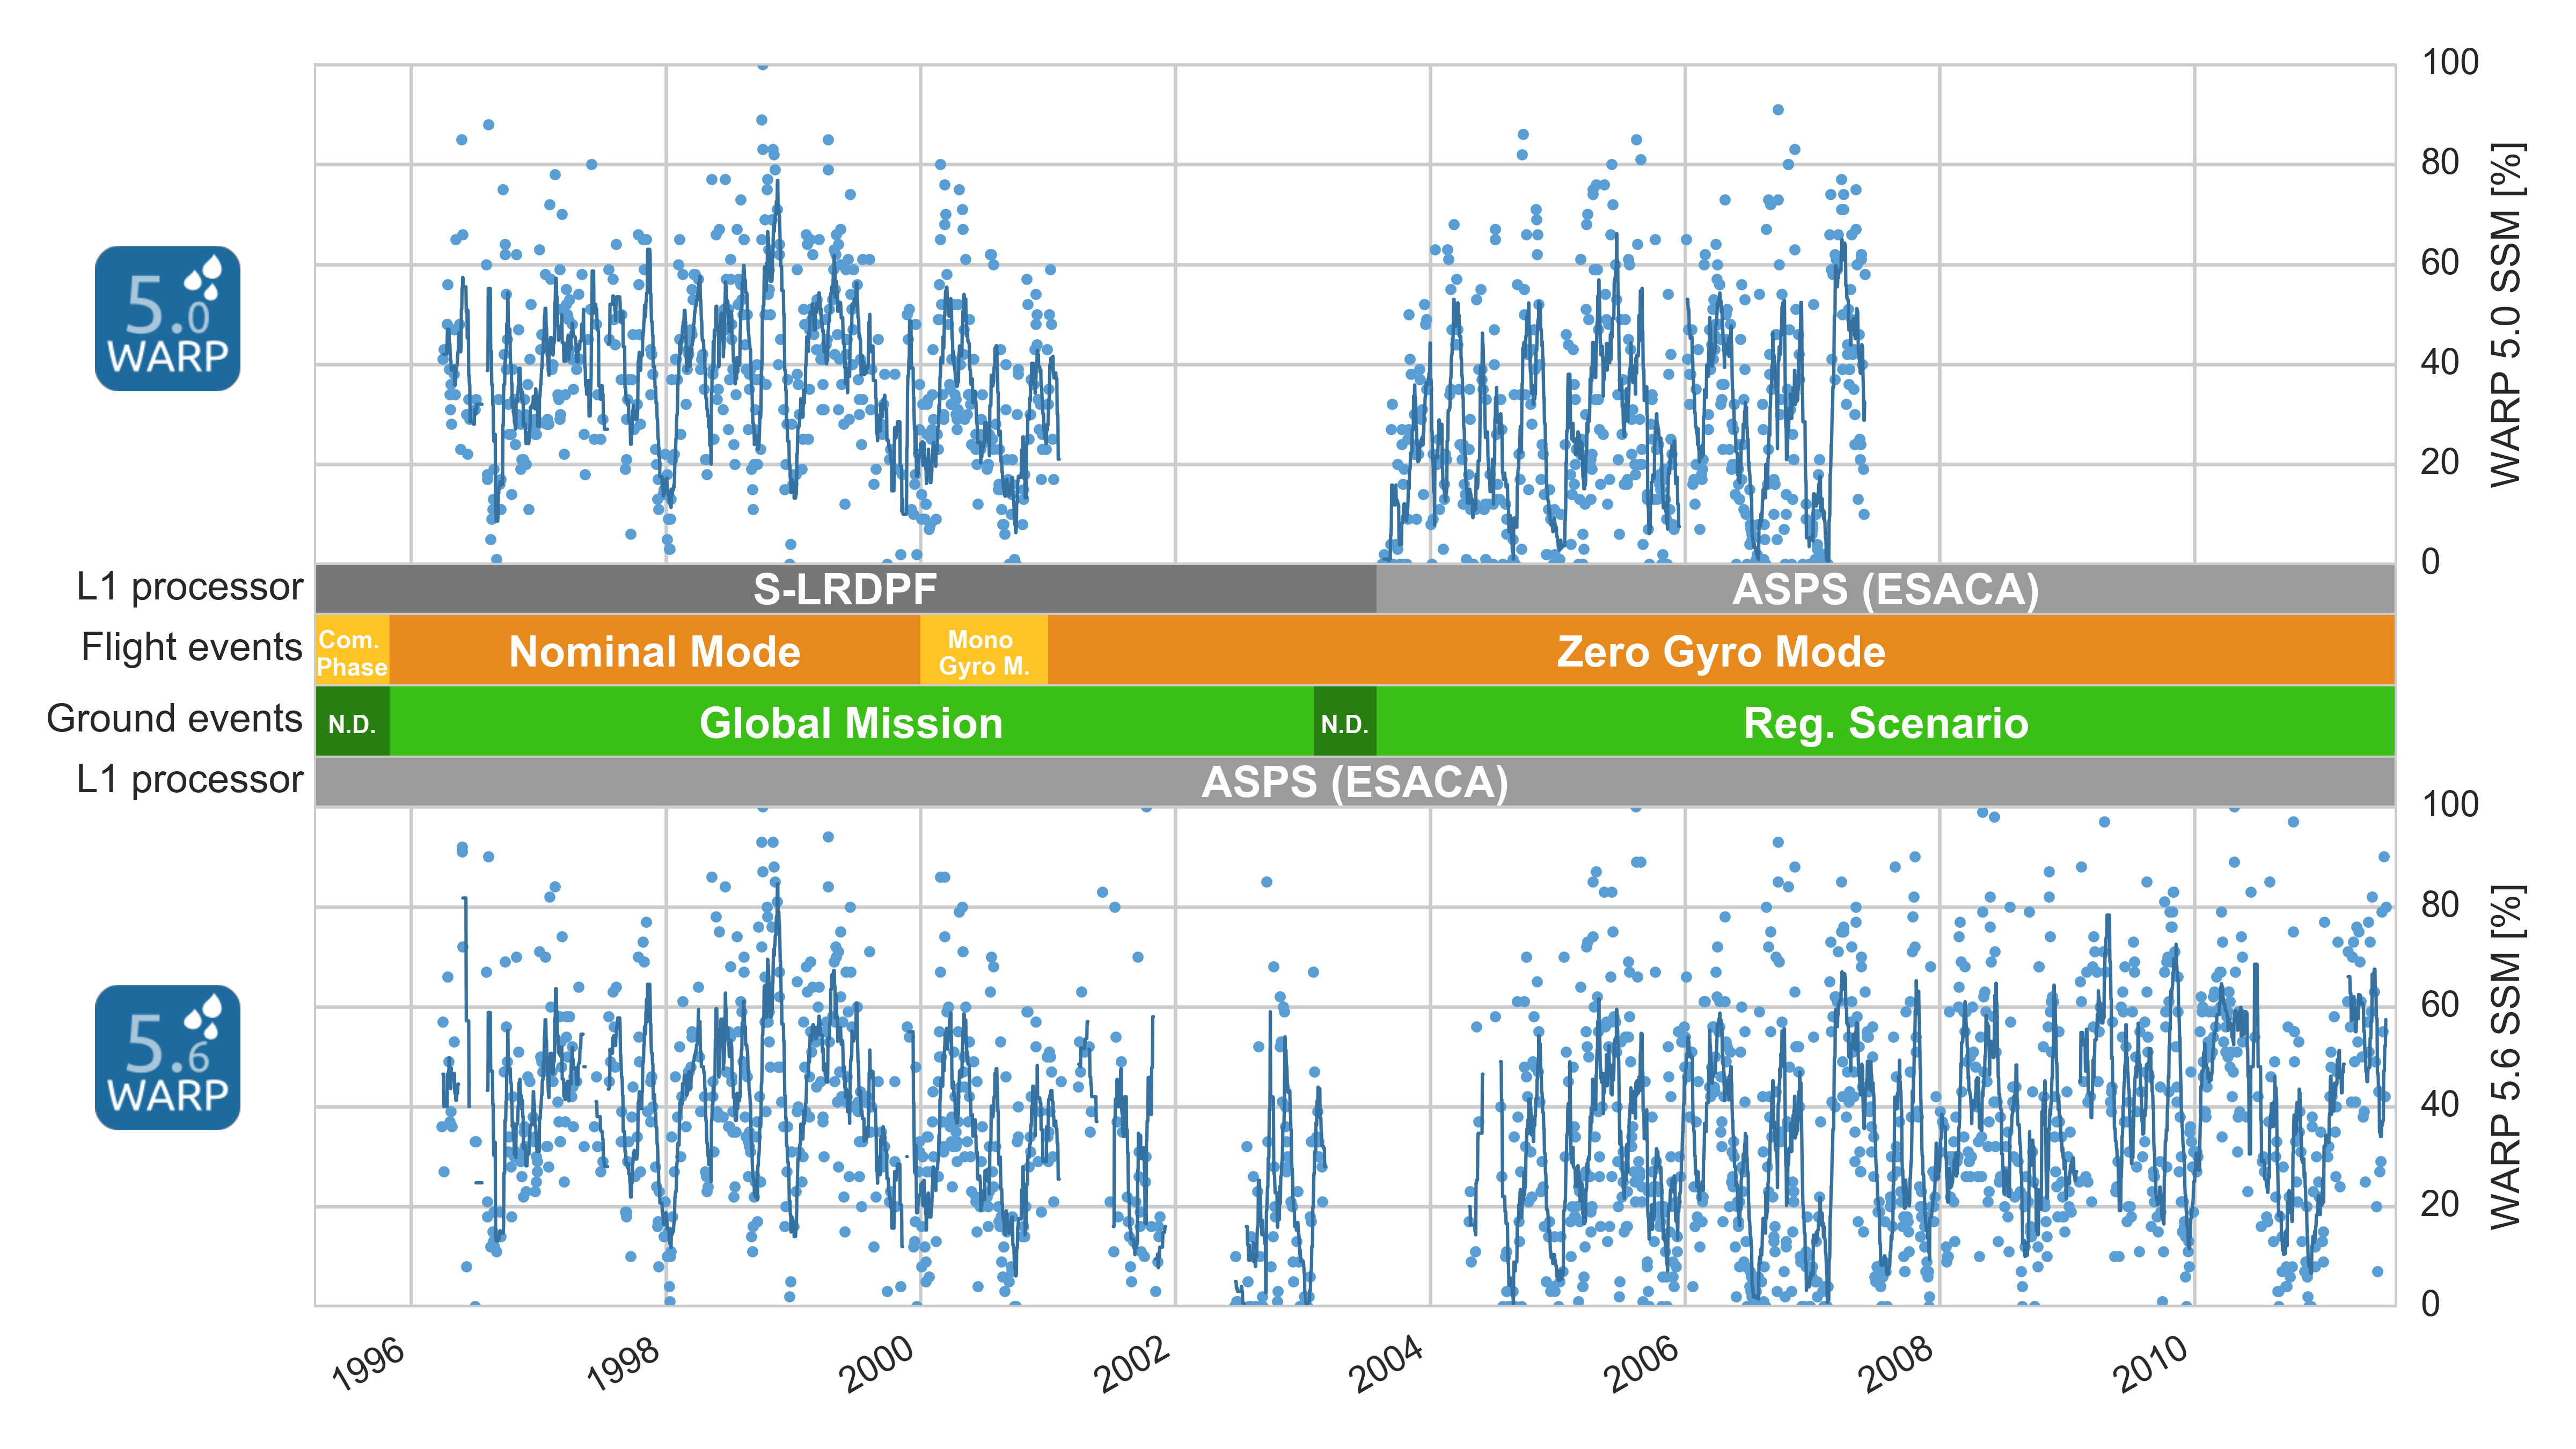
\includegraphics[width=0.45\textwidth]{figures/ERS_mission_overview.png}
        \end{tikzfigure}
      \end{center}
    }

    \block{Soil Moisture Retrieval -- Algorithm Improvements}{
      %The TU-Wien soil moisture algorithm is a physically motivated change detection approach implemented in a software called the WAter Retrieval Package (WARP).
      %Since the first release of global soil moisture observations from ESCAT, algorithmic improvements have been implemented into WARP with focus on the retrieval for ASCAT.
      
      \begin{center}
        \begin{tikzfigure}[Flow chart of the TU Wien Soil Moisture retrieval algorithm implemented in the WAter Retrieval Package (WARP). Indicated algorithmic changes and improvements are given with respect to the previous derived ESCAT SM products based on WARP 5.0.\label{figure:flow_chart}] 
          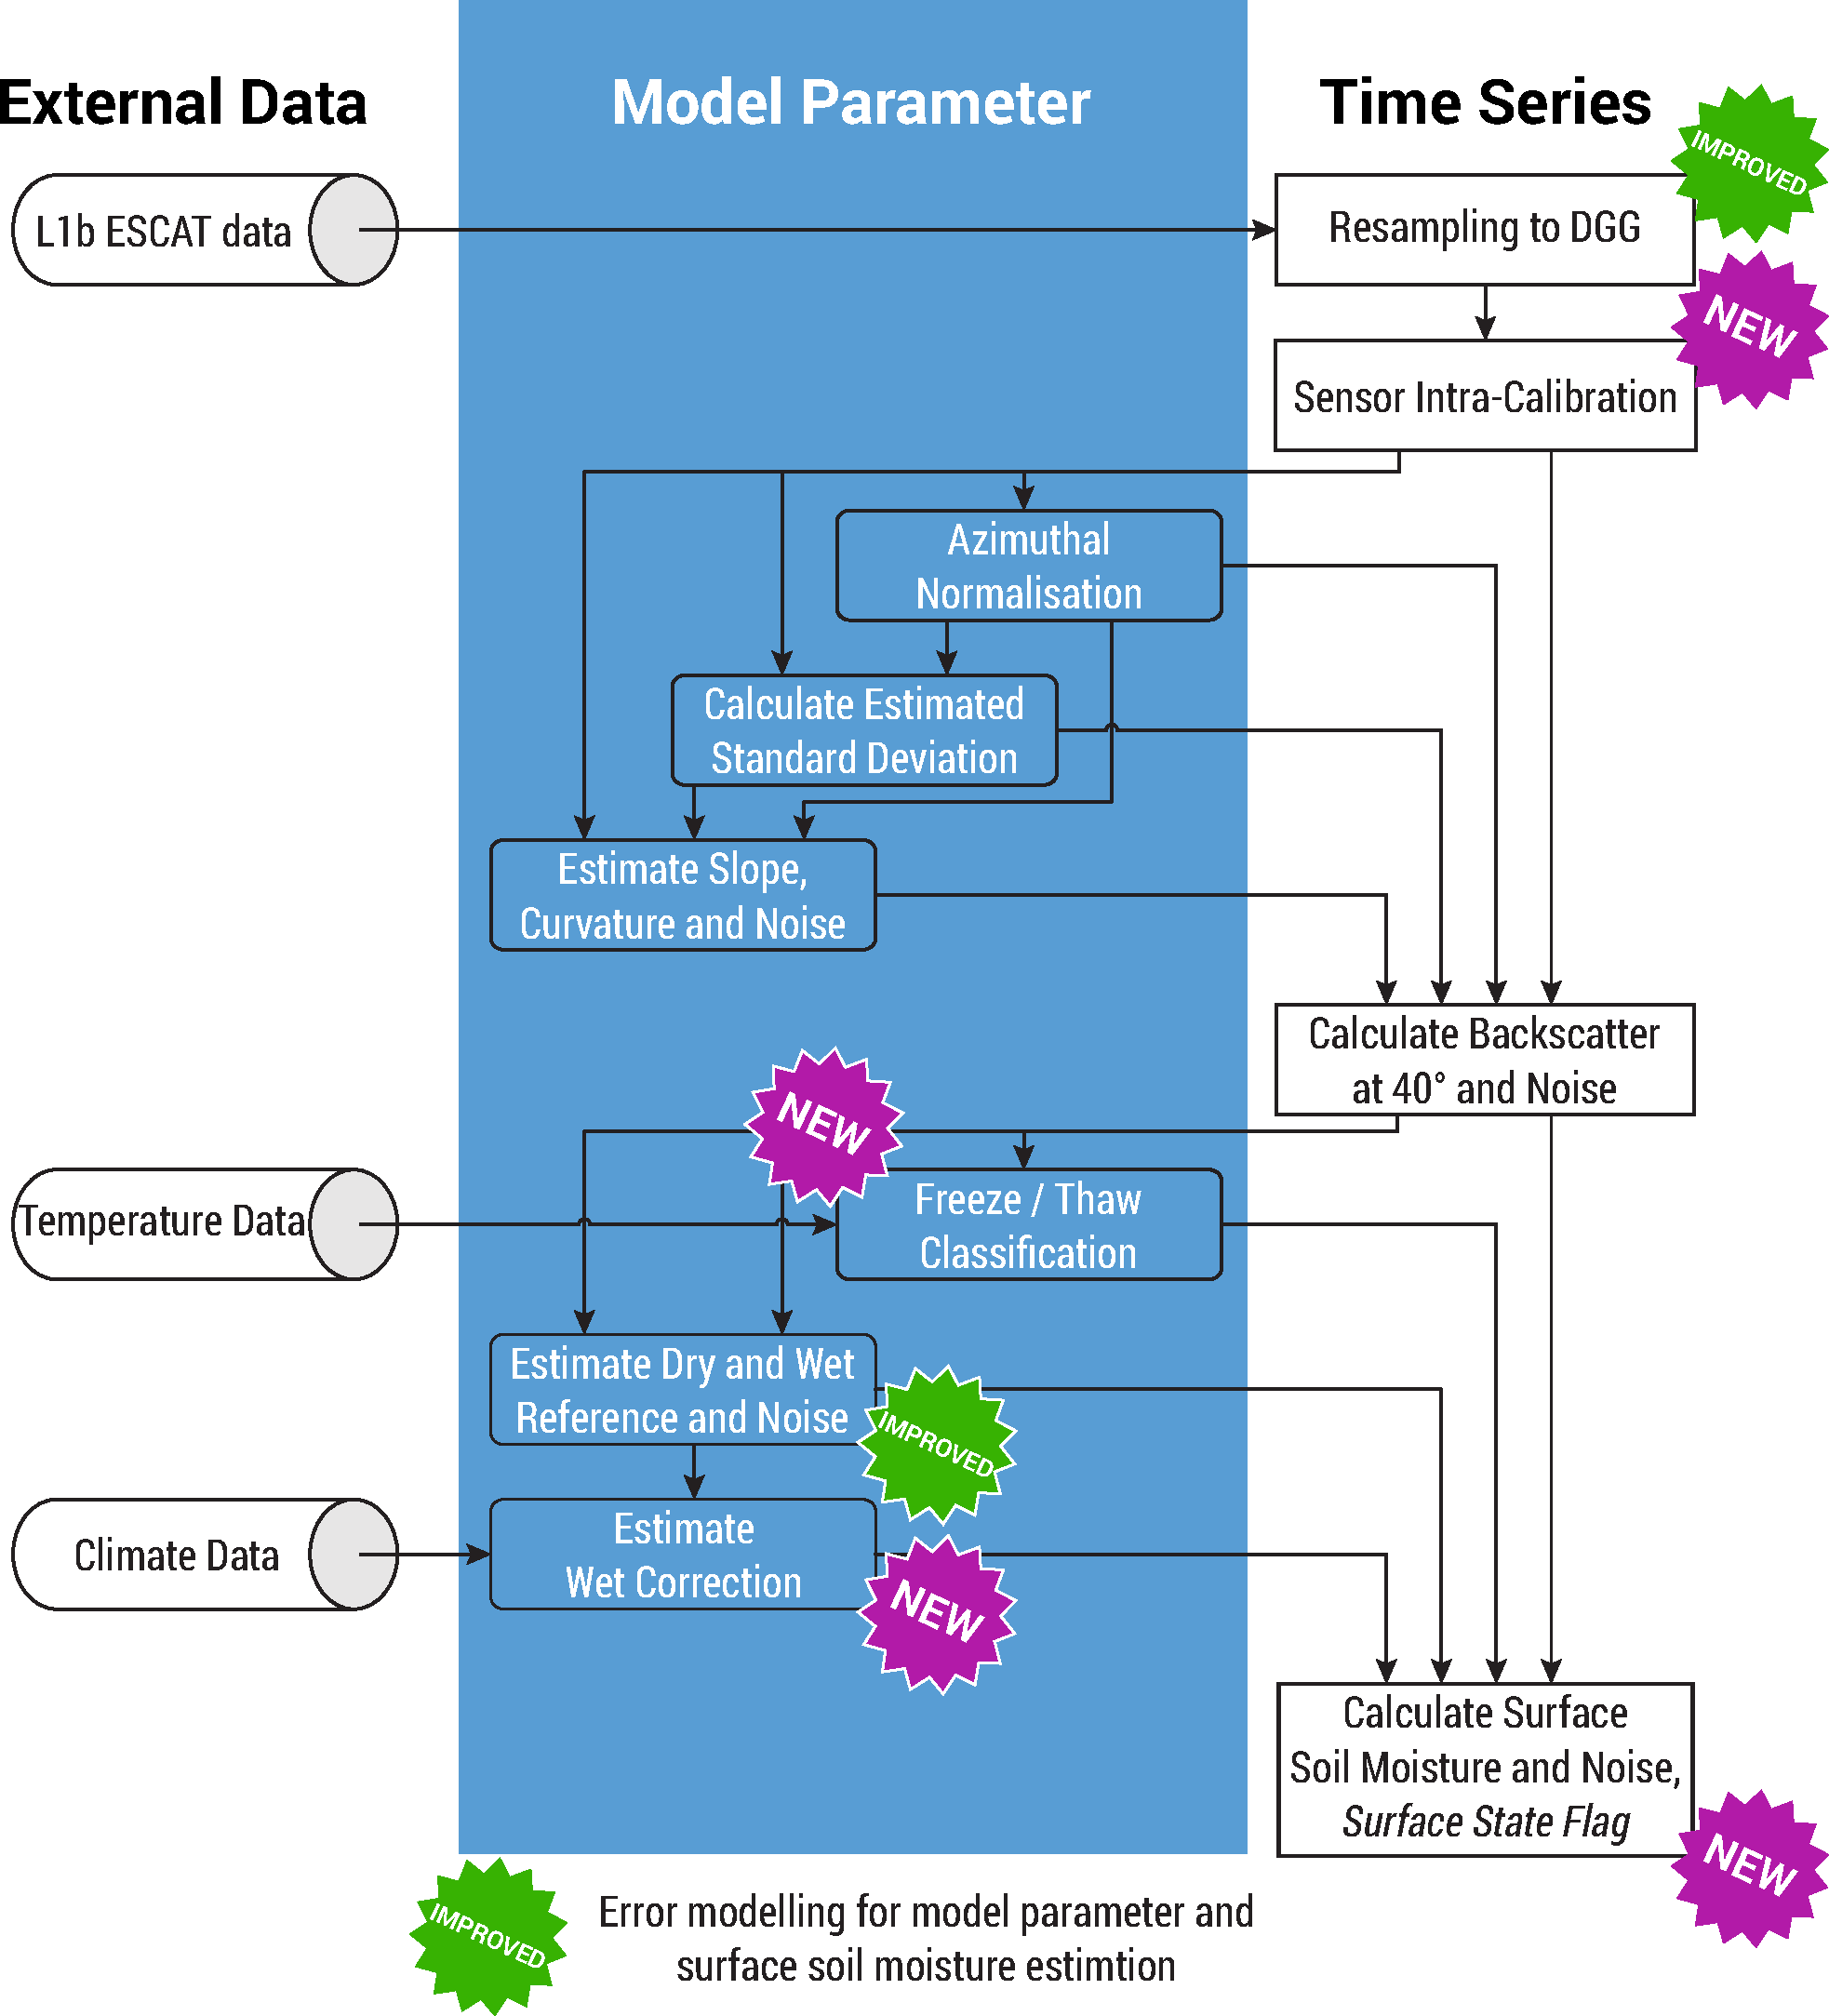
\includegraphics[width=0.9\blockwidth]{figures/WARP_processing_steps.pdf}
        \end{tikzfigure}
      \end{center}
    }

    \column{.5} 

    \block{Product Overview \phantom{Motivation}}{
      Soil Moisture products from ERS ESCAT have been re-processed resulting in a Swath-Grid and a Time-Series product to cover the wide range of applications~[see~ Figure~\ref{figure:escat_products}].
      The Swath-Grid product is aimed for NWP centers in support to NWP re-analysis and climate monitoring activities [see Figure~\ref{figure:spat_res}].
      For research and climate change studies a Time-Series product is accessible located on a discrete global earth grid [see Figure~\ref{figure:mission_events}].
      Both Soil Moisture products are available at two different spatial resolutions with a sampling of 12.5 and 25 km [see Figure~\ref{figure:spat_res}], and will be disseminated in NetCDF following the CF-conventions.\\

      \begin{center}
        \begin{tikzfigure}[ERS ESCAT Soil Moisture product generation flow chart depicting the relationship between the Swath-Grid and Time-Series products.\label{figure:escat_products}] 
          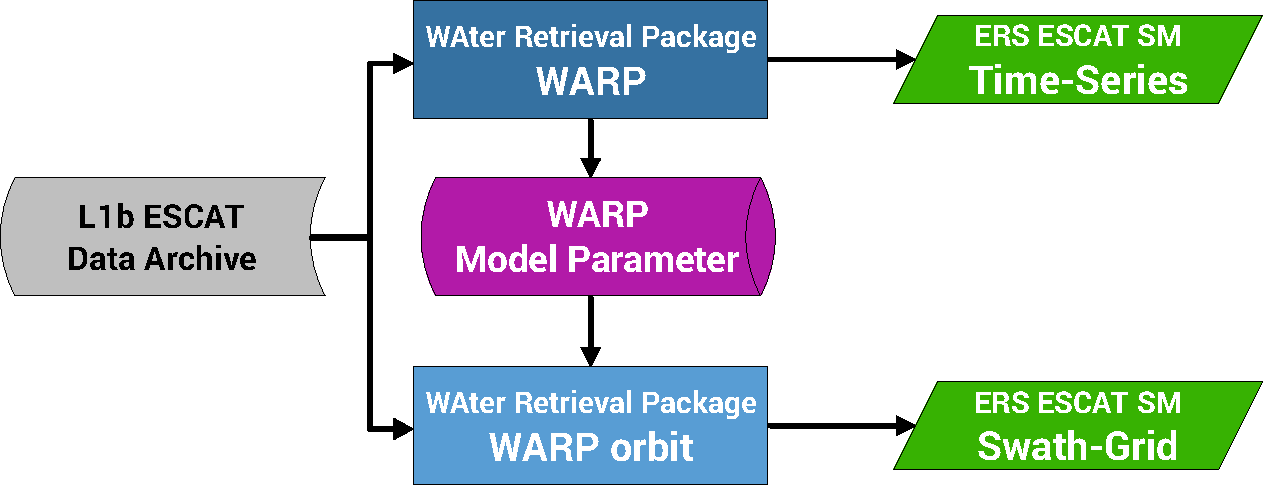
\includegraphics[width=0.65\blockwidth]{figures/WARP_WARPNRT.pdf}
        \end{tikzfigure}
      \end{center}
      
      \begin{center}
        \begin{tikzfigure}[Illustration of the different spatial resolutions of the Level 1 input dataset used for Soil Moisture retrieval at TU~Wien.\label{figure:spat_res}] 
          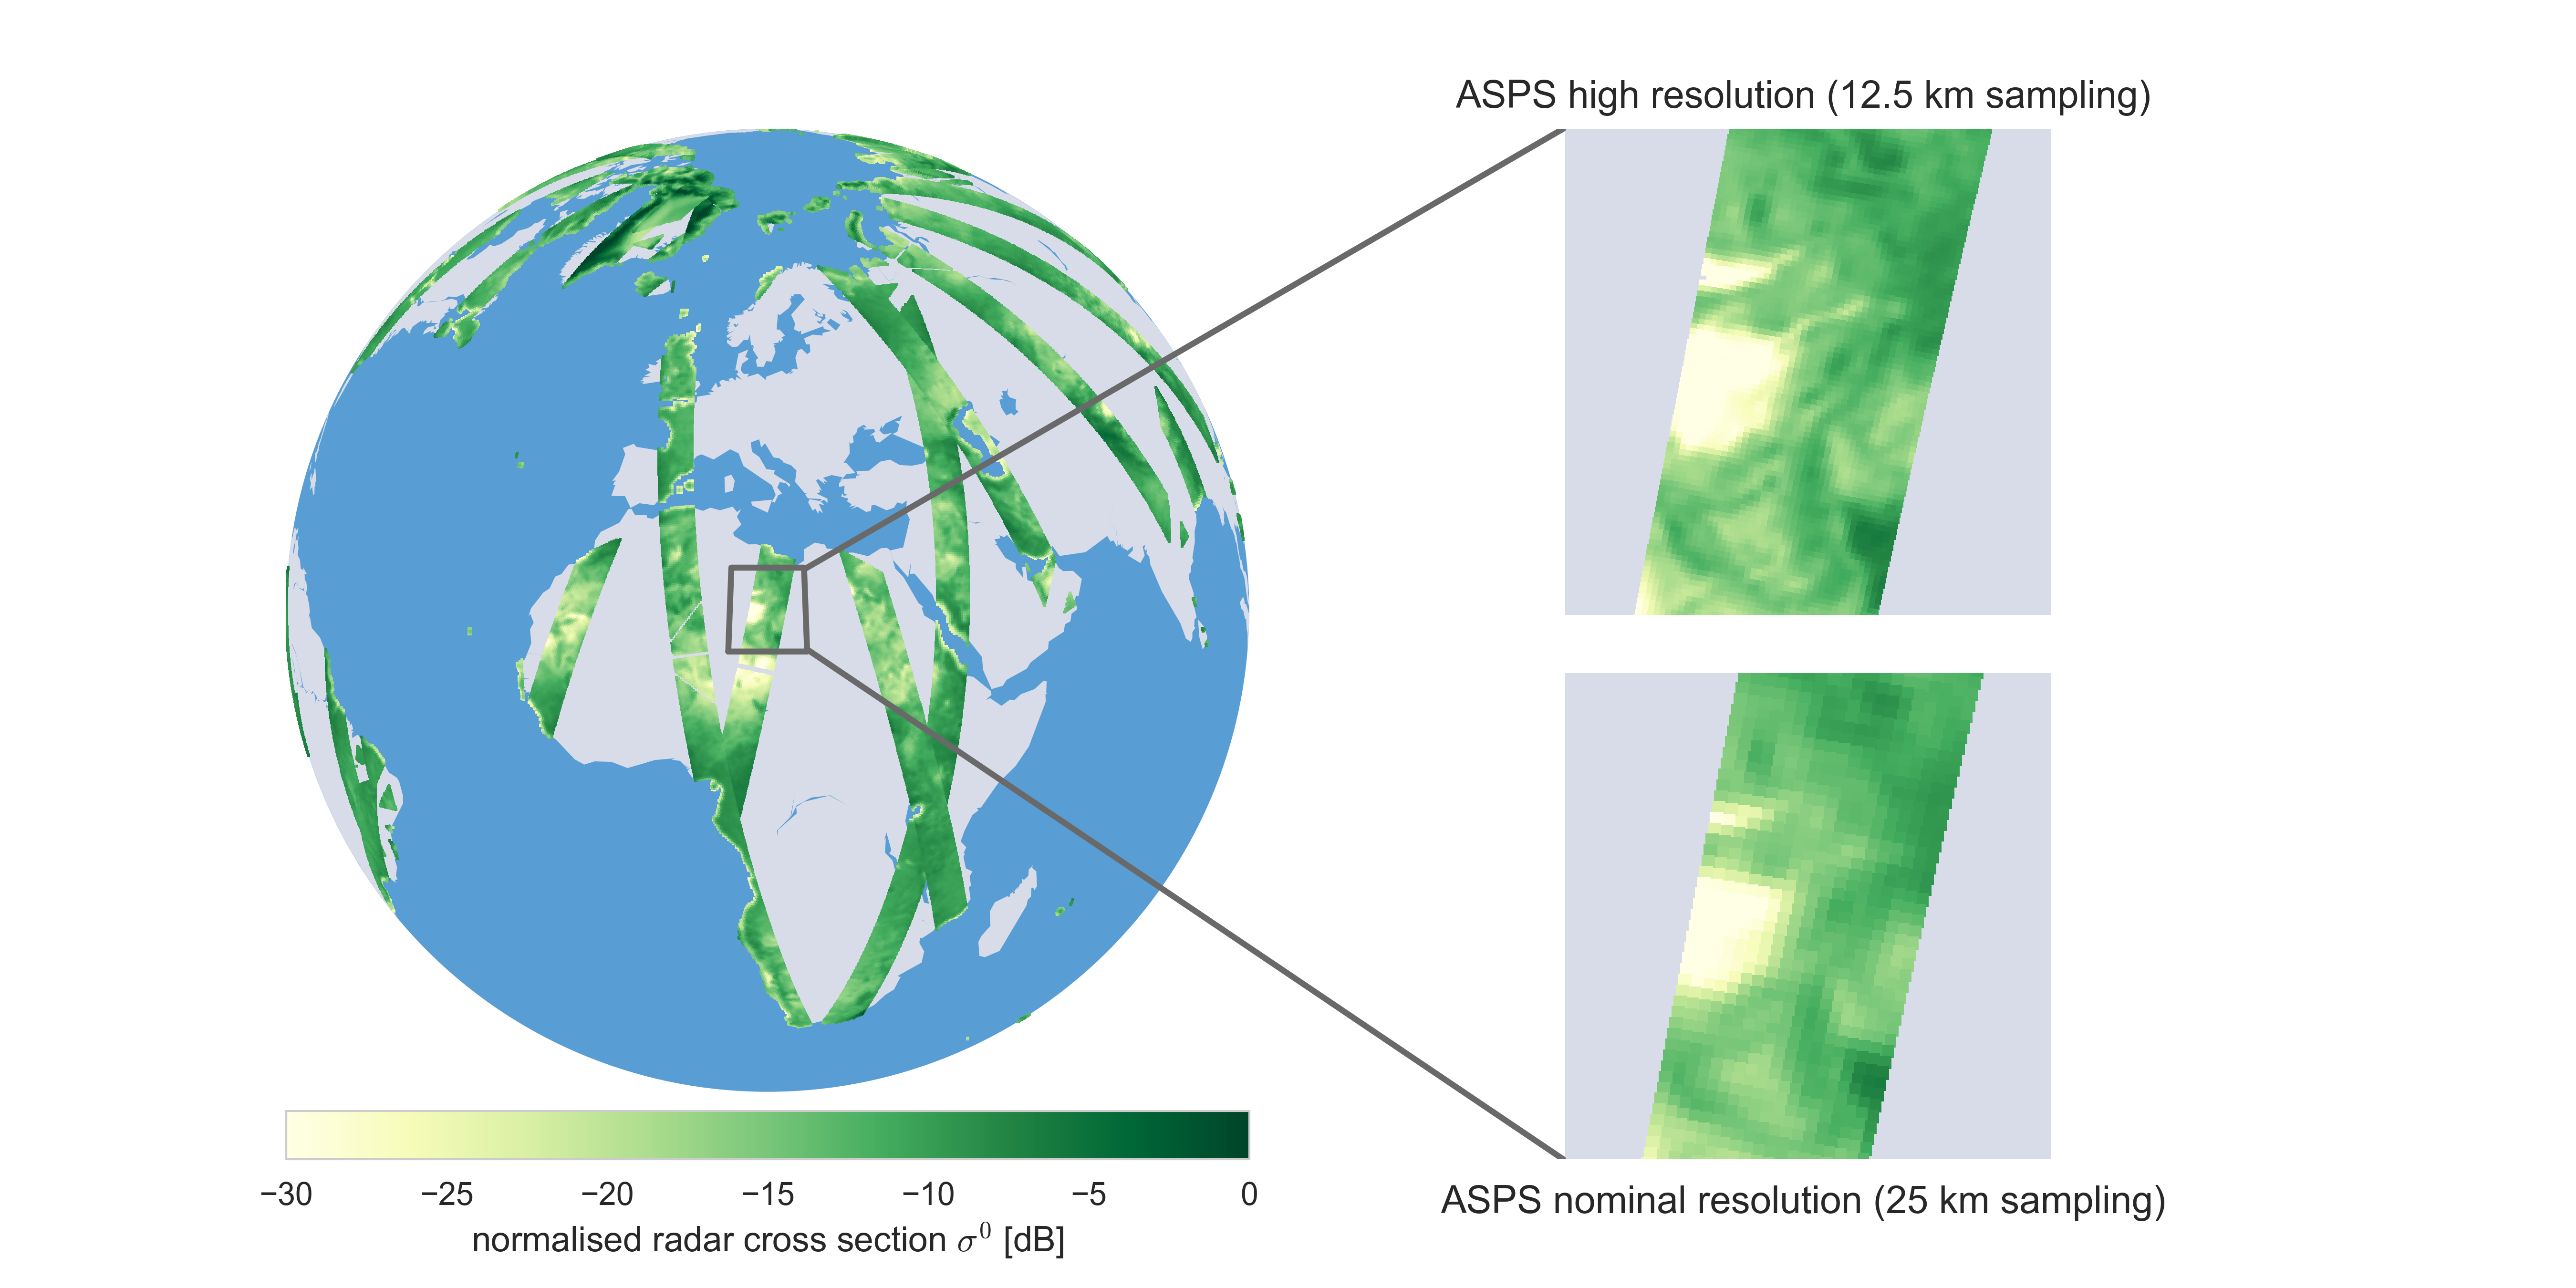
\includegraphics[width=0.9\blockwidth]{figures/ASPS_resolutions.png}
        \end{tikzfigure}
      \end{center}
 
    }

    \block{Validation Results}{
      A validation study has been carried out in order to analyze the performance of the newly computed ESCAT Soil Moisture Products.
      The products have been validated against in-situ SM observations from the International Soil Moisture Network (ISMN) [see Figure~\ref{figure:ismn_val}] and ERA-interim modeled soil moisture [see Figure~\ref{figure:lsm_val}].

      \begin{center}
        \begin{tikzfigure}[ISMN validation results utilizing Triple Collocation technique to estimate the Signal to Noise Ratio (SNR) in addition to Pearson R coefficient. Results are only shown for statistical significant correlations~(p~>~0.05).\label{figure:ismn_val}] 
          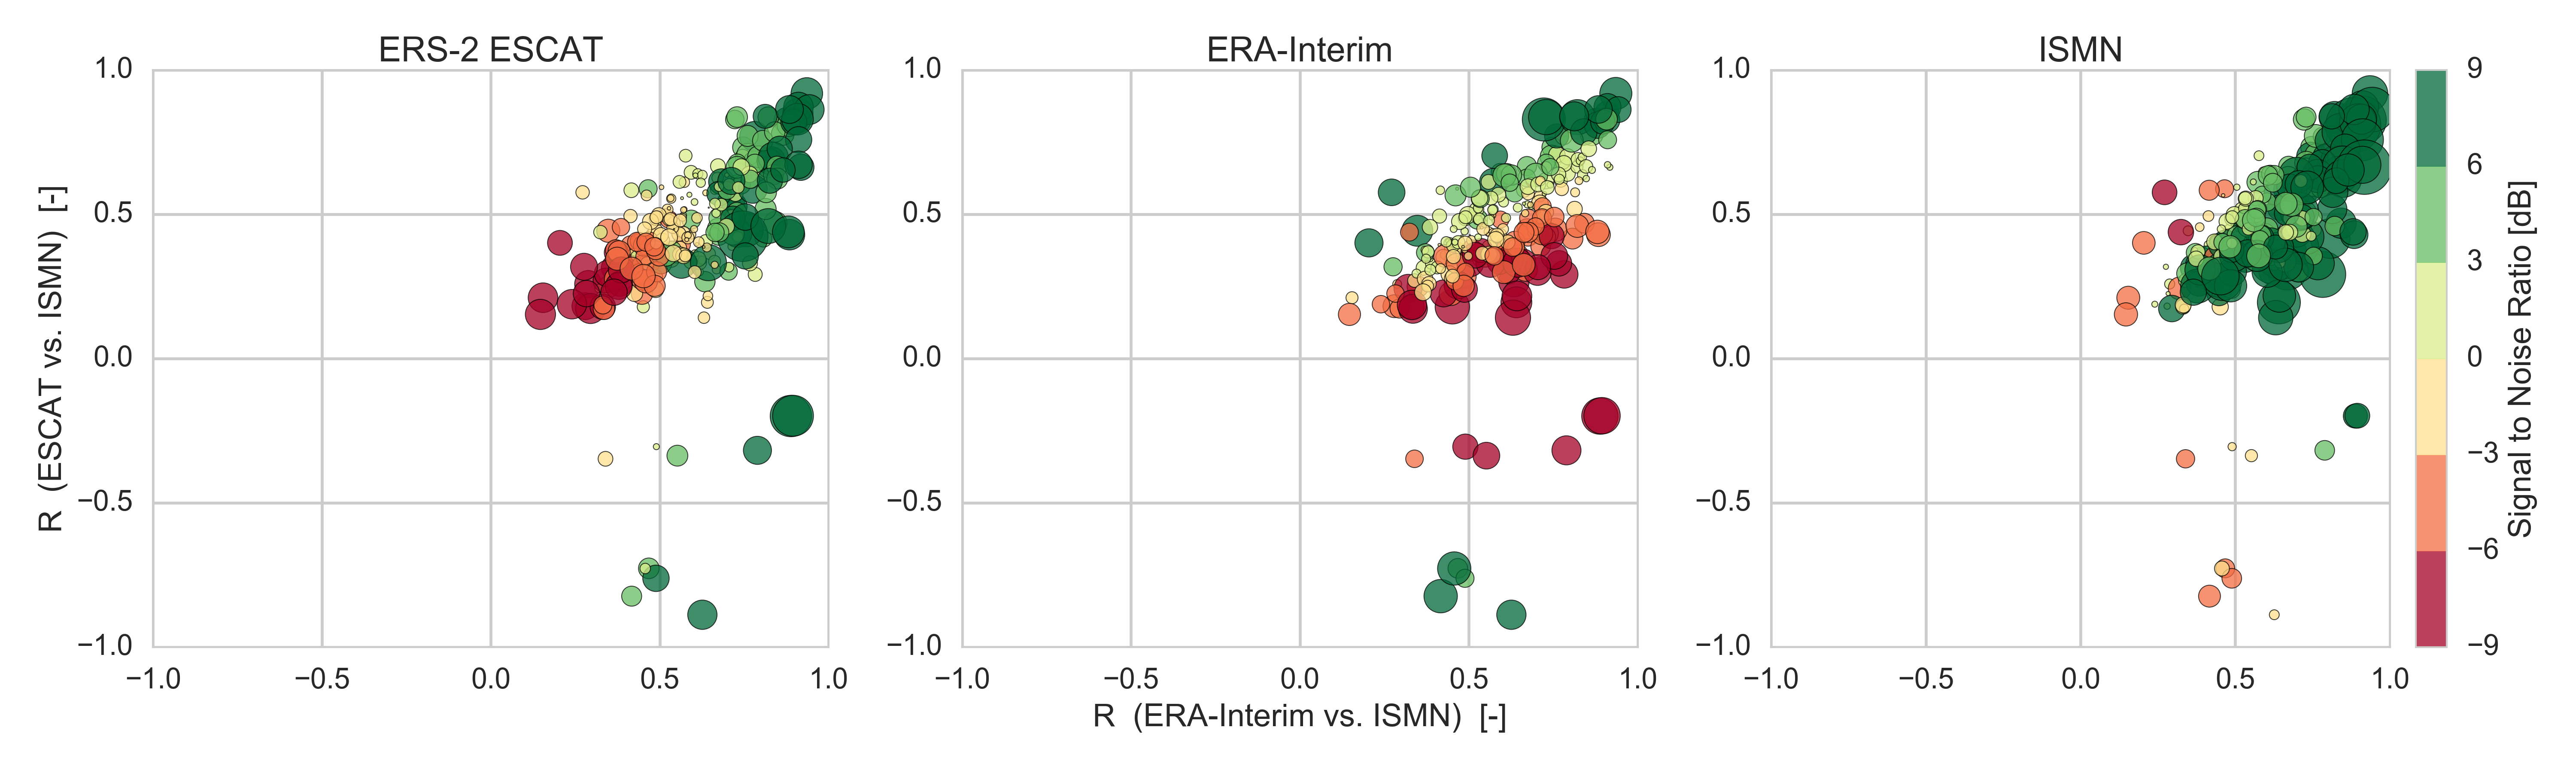
\includegraphics[width=\blockwidth]{figures/TripleCol_SNR_R.png}
        \end{tikzfigure}
      \end{center}

      \begin{center}
        \begin{tikzfigure}[Pearson Correlation Coefficient R between the derived ESCAT Soil Moisture Time-Series and ERA-interim modeled Soil Moisture. Results are only shown for statistical significant correlations (p > 0.05).\label{figure:lsm_val}] 
          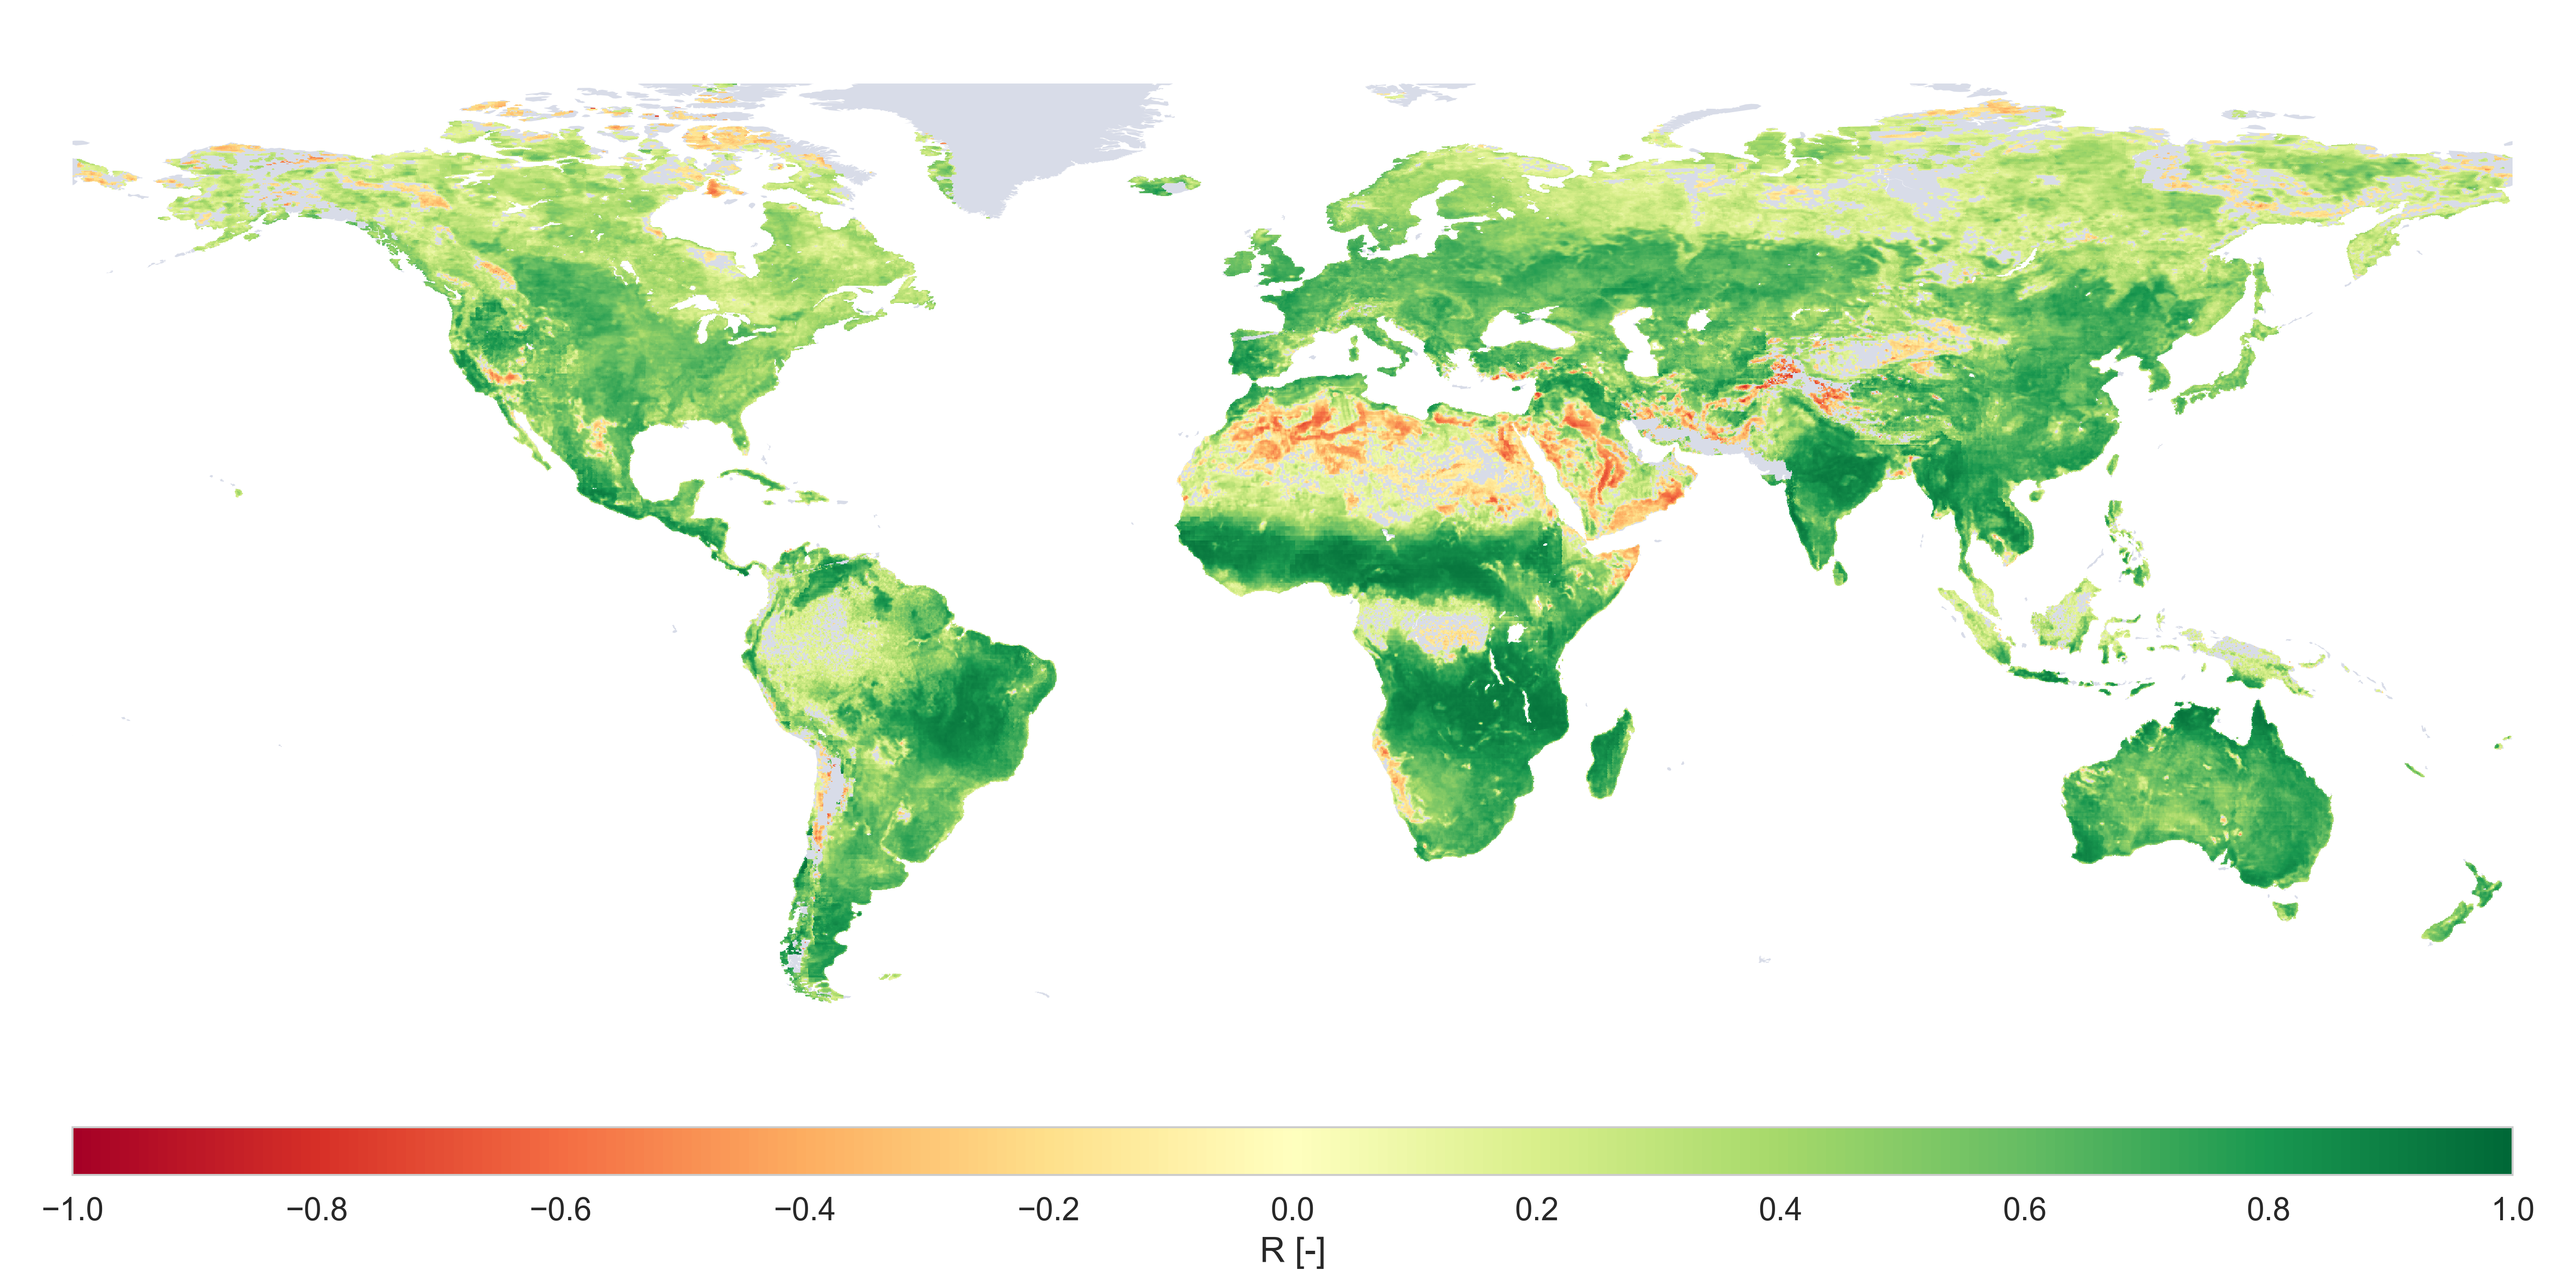
\includegraphics[width=0.84\blockwidth]{figures/WARP_SM_ERAINT_R_ALL_map.png}
        \end{tikzfigure}
      \end{center}
      
      %\begin{minipage}[t]{0.5\blockwidth}
      %  \begin{center}
      %    \begin{tikzfigure} 
      %      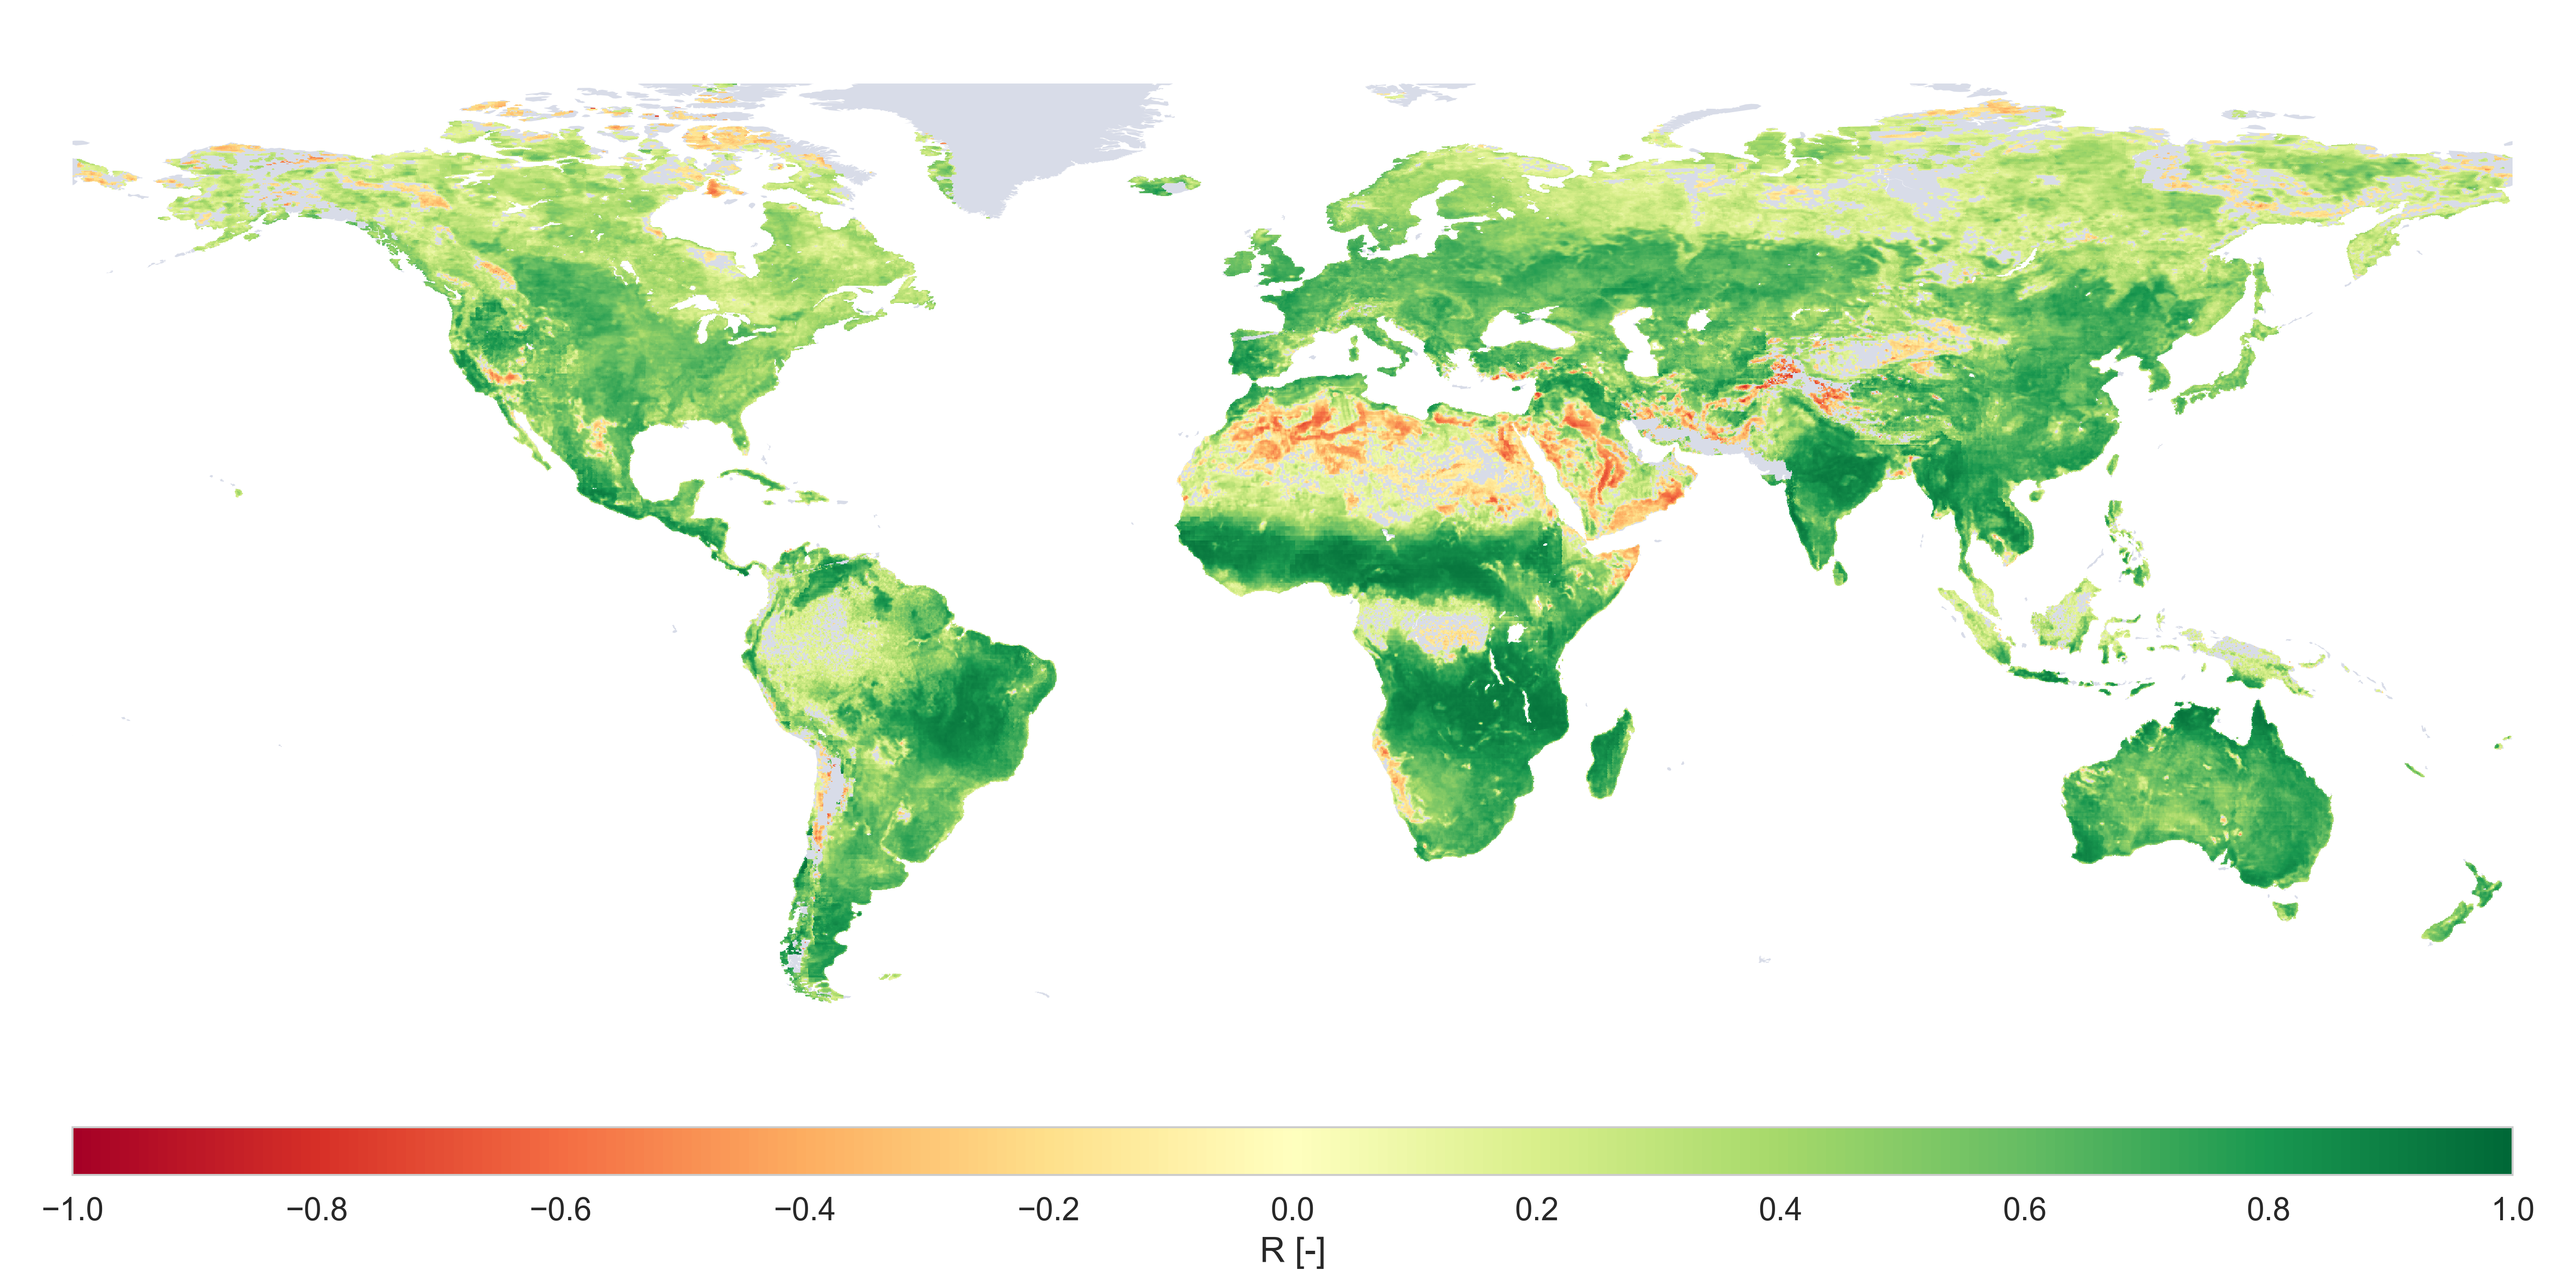
\includegraphics[width=0.49\blockwidth]{figures/WARP_SM_ERAINT_R_ALL_map.png}
      %    \end{tikzfigure}
      %  \end{center}
      %\end{minipage}
      %\begin{minipage}[t]{0.5\blockwidth}
      %  \begin{center}
      %    \begin{tikzfigure}
      %      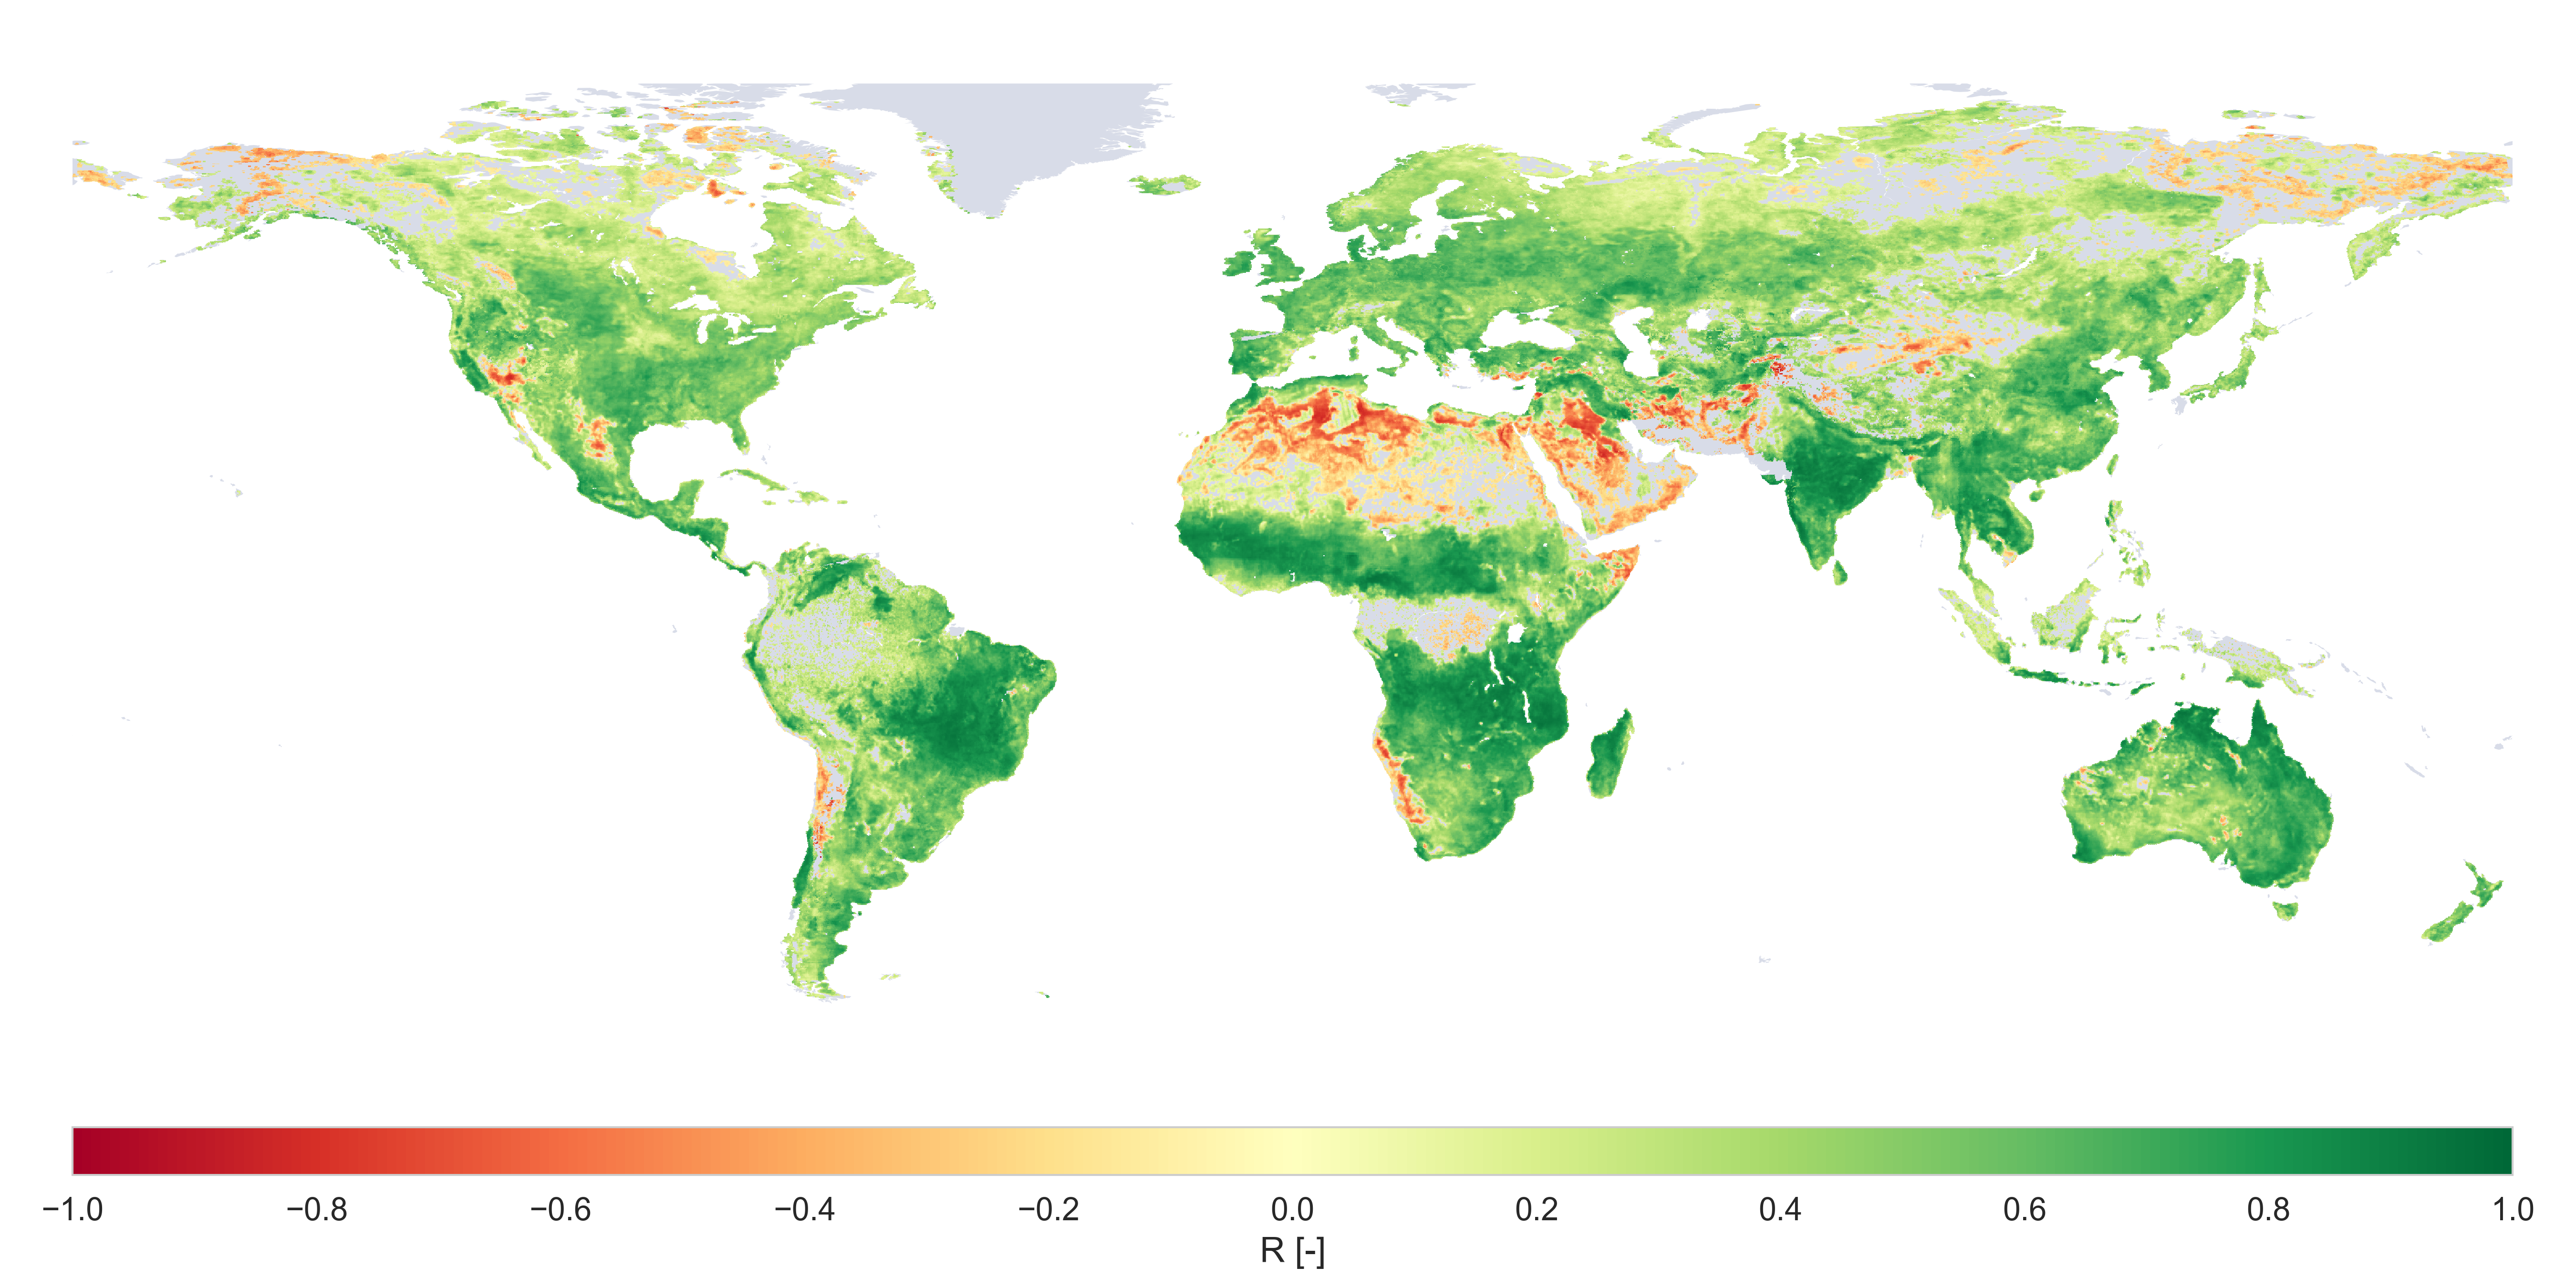
\includegraphics[width=0.49\blockwidth]{figures/WARP_SM_GLDAS_R_ALL_map.png}
      %    \end{tikzfigure}
      %  \end{center}
      %\end{minipage}
      %\begin{minipage}[t]{\blockwidth}
      %  \begin{tikzfigure}[Land surface validation]
      %    \centering
      %  \end{tikzfigure}
      %\end{minipage} 
    }
    
  \end{columns}
  
\end{document}
